
\documentclass{book}

%% Paquetes
\usepackage[spanish,mexico]{babel}
\usepackage{graphicx}
\usepackage{multirow}
\usepackage{multicol}
\usepackage{float}
\usepackage{array}
\usepackage{amsmath}
\usepackage{mathtools}
\usepackage{amsthm}
\usepackage{amssymb}


%% Comandos para Theoremas
\newtheorem{dem}{Demostracion}
\newtheorem{teo}{Teorema}

%% Titulo
\title{\textbf{PRÁCTICA 1}}
\author{\textbf{Julian, Erick, Sergio, Luis}}
\date{\textbf{\today}}

%% Fonts
\renewcommand{\familydefault}{\rmdefault}
\begin{document}
\maketitle
\tableofcontents


\chapter{Julián Rosas Scull}

\section{Pasatiempos}

\large
Algunos de mis pasatiempos favoritos son realizar \textbf{\textit{Slackline}} y nadar.
\\

\textit{Slackline} es un deporte que invlocura el caminar sobre una cuerda, la cual se encuentra amarrada en medio de dos árboles, éste mismo se enfoca en
la capacidad de mantener el equilibrio. Por otra parte, \textbf{nadar} es un pasatiempo en el cual pude llegar a competir regionalmente contra otros clubes.
\\

De igual manera, me encanta jugar videojuegos (The Last Of Us siendo mi juego favorito) al igual que escuchar música, especialmente música alternativa,
como Radiohead (mi banda favorita) y Bjork.
\\

\begin{figure}[H]
  \centering
  
\includegraphics[scale=0.1]{./radiohead.jpg}
  \caption{Radiohead :b, mi banda favorita.}
  \label{radiohead}
\end{figure}

\clearpage

De Igual manera que la imagen \textbf{\ref{radiohead}}, otro de mis pasatiempos es:

\begin{figure}[H]
  \centering
  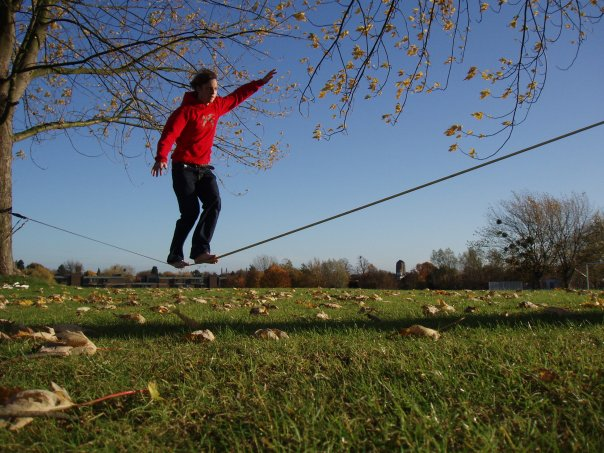
\includegraphics[scale=0.3]{./slackline .jpg}
  \caption{slackline}
  \label{slack}
\end{figure}

El cual (como ya mencioné anteriormente y se observa en la imagen \textbf{\ref{slack}}), se tiene que caminar a traves de una cuerda.
\\

Igualmente me encanta ver series y películas, mi película favorita (o la que mas me ha llegado por el momento) es \textit{Whiplash}.

\section{¿Por qué escogí estudiar Ciencias de la Computación?}

Una de mis mayores pasiones desde que era pequeño, fueron los videojuegos, en especial, los que storytelling. Gracias a éstos fue la primera vez
que quize involucrarme en la programación y en el desarrollo de los mismos.
\\

Años despues, al tener contacto con la interfaz y el lengiaje Visual Basic en 2-3ro de secundaria, me llamó aun más la atención la programación y
cómo las variables se interrelacionaban, además que era algo inimginable, estaba haciendo que una (o varias) pelotitas se movieran con algo que yo creé. Desde ahí,
mi fascinación sobre esta carrera.
\\

Tiempo despues me empecé a involucrar en otros lenguajes de programación (Python, por obvias razones, siendo el que mejor controlo) y haciendo mini proyectos, tales
como blogs o páginas web utilizando Django e interpretadores como HTML y CSS.
\\

De igual manera, otra razón por la que escogí Ciencias de la Computación fue el enfoque matemático que tiene y (como buena Ciencia) el enfoque de demostrar, ya que
desde la secundaria y la preparatoria, me fascinaban hacer demostraciones de fórmulas y de teoremas, observar como iba divergiendo una simple expresión a una
fórmula que es utilizada mundialmente, era algo que nunca había experimentado. Al igual que la materia Lógica, siempre fue una de mis favoritas.
\\

\section{Demostración de mi teorema favorito}


\begin{teo}[Fórmula de la parabola vertical en el origen]
  La fórmula se define como:
  \[
  \left(x^2=4py \right)
  \]
  
\end{teo}

\begin{proof}
  \begin{enumerate}
  \item Para saber los elementos de la misma, tendremos que trazarla:
  \begin{center}
    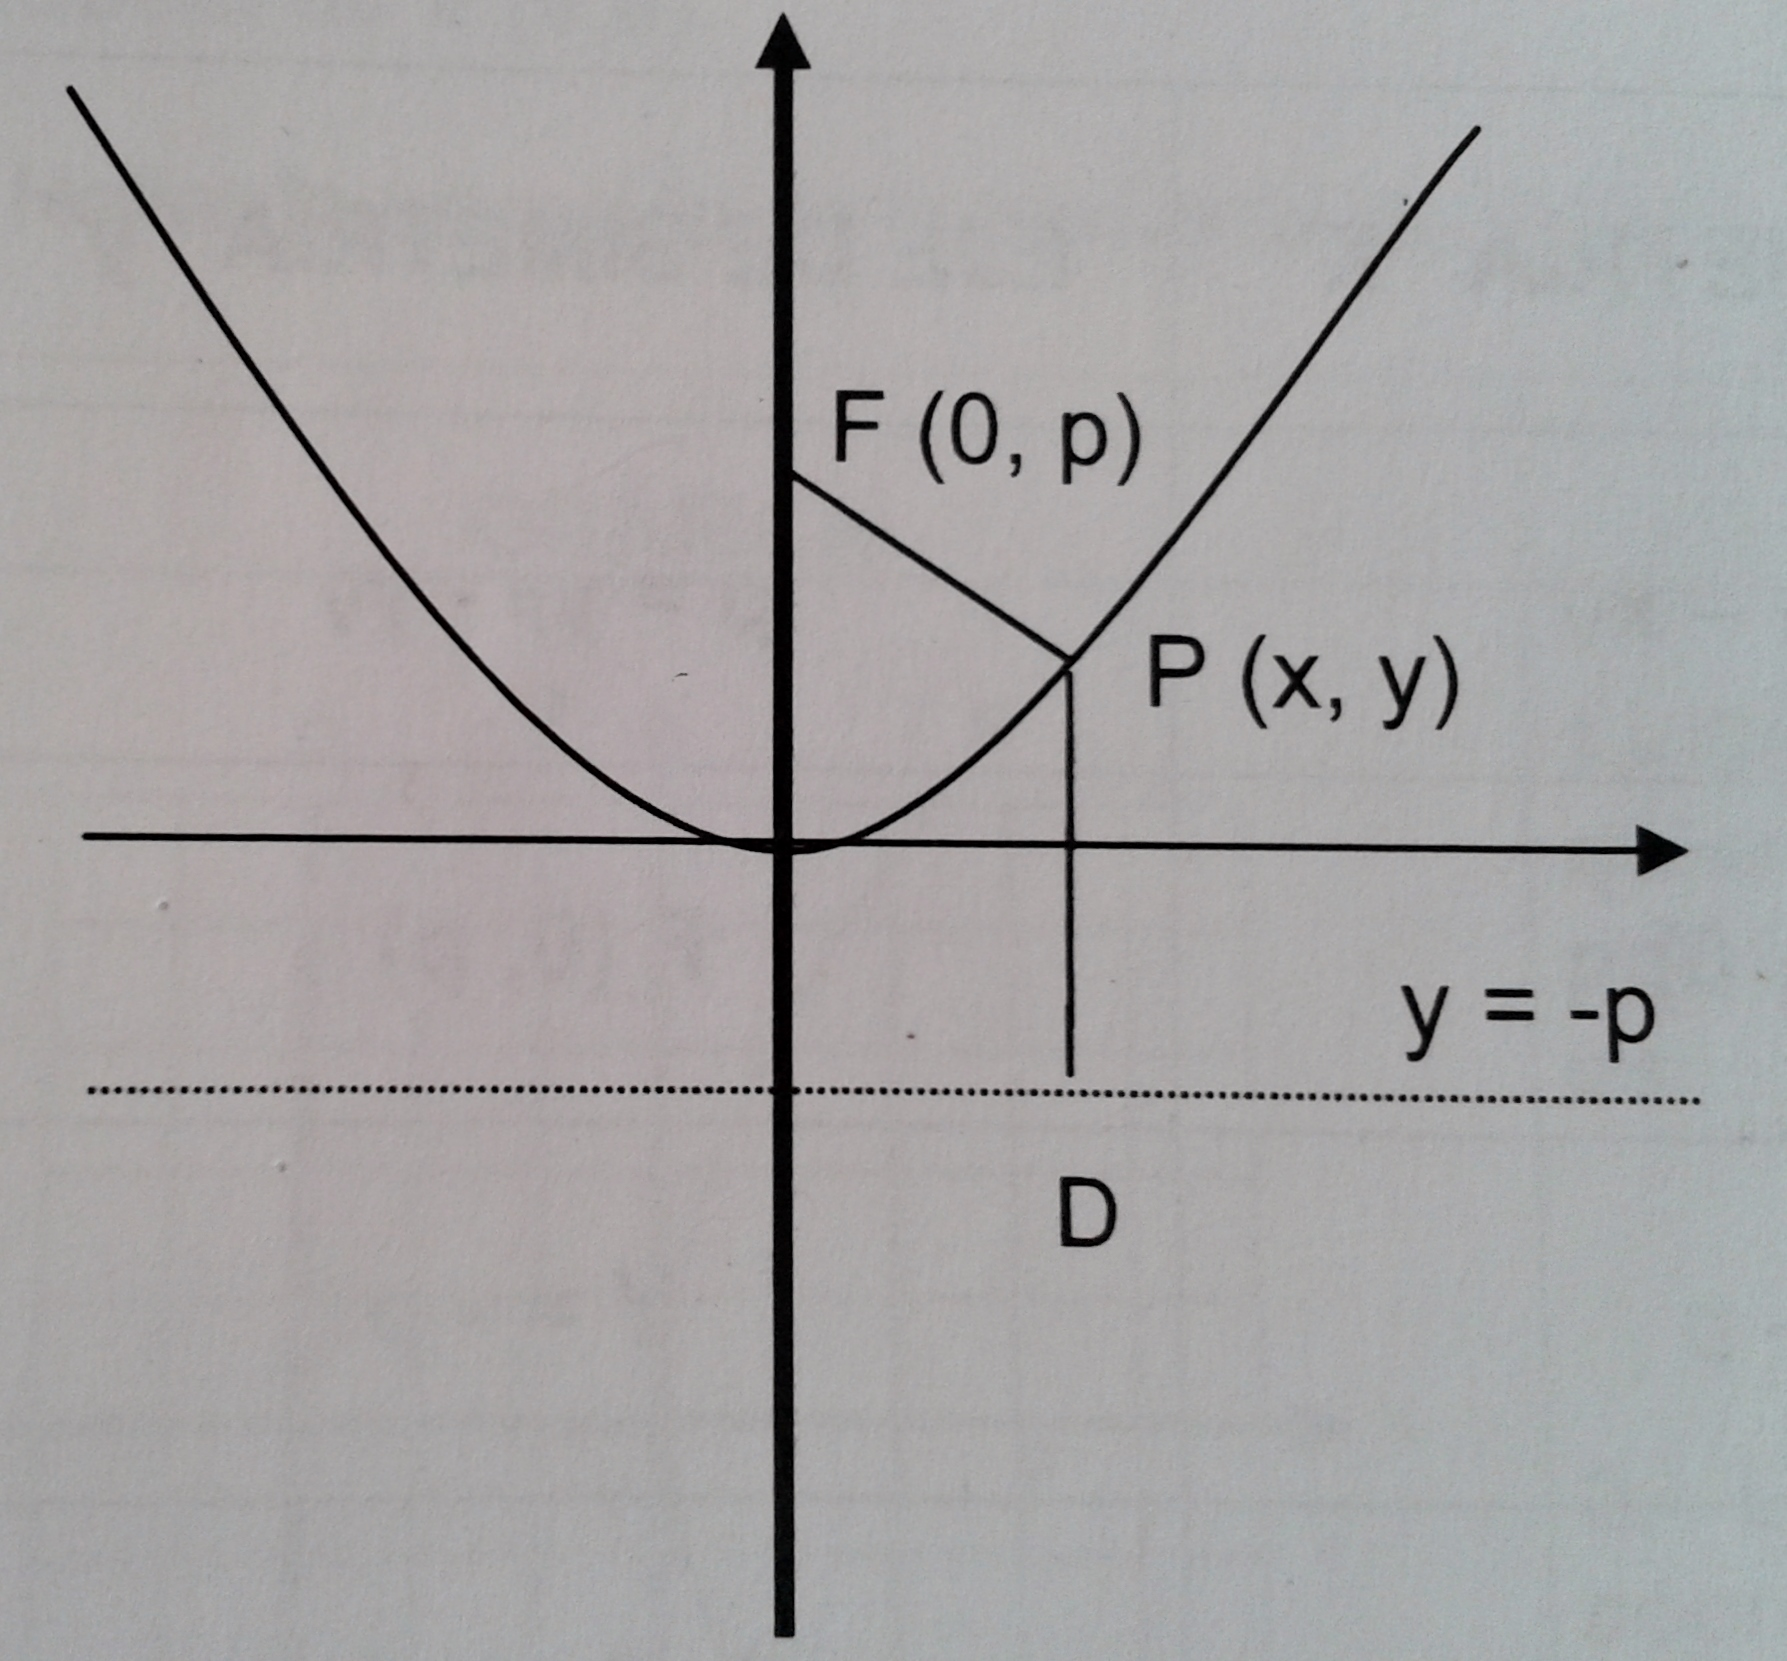
\includegraphics[scale=0.1]{./parabola.jpg}
  \end{center}
\item De tal manera que tenemos $D:$ refiriéndose a la directriz, $F:$ refiriéndose al foco, $P:$ refiriéndose a un punto cualquiera de la parábola con coordenadas
  $(x,y)$. 
  \end{enumerate}
\end{proof}  



\end{document}
